
\documentclass[10pt, twocolumn]{article}
\usepackage{amsmath}
\usepackage{siunitx}
\usepackage{graphicx, float}
\usepackage[plain]{algorithm}
\usepackage{url}

\topmargin=-0.45in
\evensidemargin=0in
\oddsidemargin=0in
\textwidth=6.5in
\textheight=9.0in
\headsep=0.25in


\title{Group Design Project: Formal Report}
\author{Evolution Acoustics: Alex Booth}



\begin{document}
    \maketitle
    \begin{abstract}
        \it
        {
            This report details the design considerations and process for a detached multipurpose recording studio.
            Considerations for the construction's dimensions and materials are detailed, as well as steps to correct any issues that may arise in the acoustic environment.
            A case study of a real life location provides problems that are explored in the report.
            A conclusion section analyses the strengths and weaknesses of the design.
            Instead of a single adopted design theories and principles section, literature and theory will be discussed where applicable, alongside results and design principles.
        } 
    \end{abstract}
    \section{Introduction}
    The aim of this report is to detail the design of a music studio space from the ground-up for educational purposes.
    The building and the spaces within were designed by following a criteria, that the project manager has provided. 
    The manager's criteria is as follows:
    \begin{enumerate}
        \item Detached recording house comprising of 6 varied studios.
        \item Next to a busy "A" road.
        \item 6 live rooms, 4 control rooms and functional spaces such as storage rooms, reception area, technician's office and practice rooms.
        \item Constructed using prefabricated modular building technologies. Should be sub-contracted to a suitable manufacturer. Prefabricated building should meet the reasonable acoustic requirements.
    \end{enumerate}
    My main role in this design process was to set room acoustical targets, predict room modes, and explore how to achieve these target through numerical analysis and calculations.
    \section{Location case study}
        Choosing a real-life location for our project was a conscious choice for our group.
        We decided that instead of making up prospective acoustical and spatial challenges, working around strict environments that cannot be changed would have greater realism, and would enable us to spend a greater amount of time on finding and developing solutions to the problems these strict constraints presented us.
        A plot of land was chosen: 160 Graham Road, Hackney, London.
        It is adjacent to residential areas, two train lines, and a busy road, and thus presented us with an ample supply of problems to plan for and overcome, especially the noise created by the road and the trainlines.
        \begin{figure*}[ht]
            \centering
            \centerline{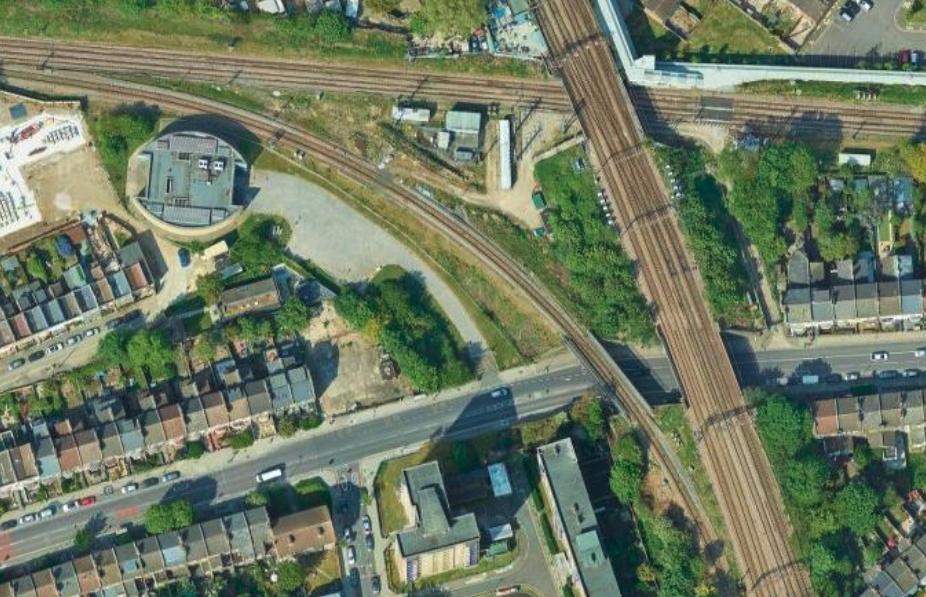
\includegraphics[scale=0.5]{resources/160 Graham Road.png}}
            \caption{Satellite Image of 160 Graham Road, E8}
            \label{graham}
        \end{figure*}
    \section{Background and Theory Basis}
        \subsection{Necessary Assumptions}
            For ease of design, we must first make some assumptions.
            Firstly, we must assume that any planning permission will be granted; the case study takes place in an inner London borough, so the planning permission process may be arduous to map out.
            For the sake of brevity, it was decided to omit this consideration.
            We assume the speed of sound in air $c=343$, the threshold of human hearing $p_{ref}$ to be $20*10^{-6}\si{\pascal}$.
        \subsection{Educational facilities}
            Any building that facilitates or is used for educational purposes must comply to the education building regulations specified by the government.
            These specifications are laid out in Building Bulletin 93 (BB93): Acoustic design of schools - performance standards.
            The importance of acoustic considerations is given by the National Education Union: "Noise from adjacent rooms disrupts the learning process, especially during quiet reading times or test-taking"\cite{NEU}
            The NEU further states the importance of tuning the reverb time of a classroom environment such that the teacher can be heard clearly at any point the classroom, but also so that the conversation of students does not descend into cacophony.
            In BB93, a table of appropriate $L_{AEQ}$ values are given for various classrooms.
            In this context, only the music rooms and common rooms entries are relevant.
            \begin{figure*}
                \centering
                \centerline{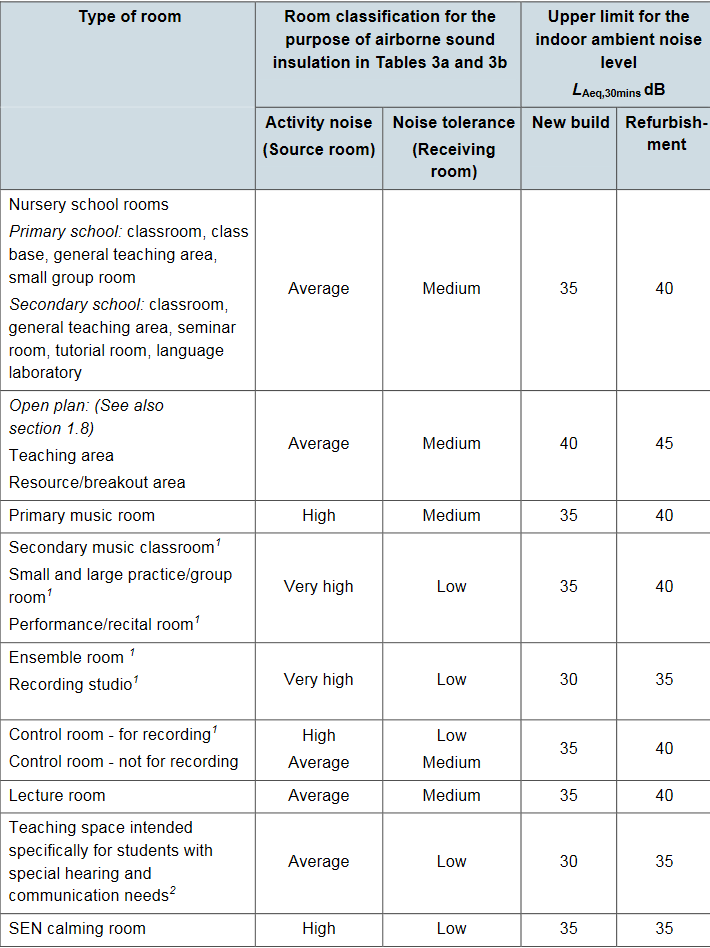
\includegraphics[scale = 1]{resources/BB93.png}}
                \caption{The tabulated $L_{AEQ}$ requirements of an educational environment}
                \label{BB93}
            \end{figure*}
            In Fig.\ref{BB93} it can be seen that classrooms and general teaching rooms have a matching ambient noise requirement to lecture rooms.
            The live room in the studio complex can function not only as a live room for large ensemble recordings but also as a class / lecture room.
            Furthermore, the control rooms, isolation rooms and foley rooms will be able to function as SEN calming rooms and teaching space for those with special hearing a communication needs, as they provide the acoustically 'dead' environment specified in the table, with a low ambient noise level.

        \subsection{Music and Recording Facilities}
            Mainstream music education at a secondary level primarily focuses on basic music theory of rhythm, timbre and tone, along with basic music technology requirements.
            In the live room, large performances and lectures can take place, whilst students wishing to practice any instruments can use the iso and control rooms to be isolated from the noise of the live room, and vice versa for the students in the live room.
            For later years of education, the studio will be able to function as an excellent teaching environment for students of sound recording techniques and studio production, with three separate control rooms and one mastering room all equipped such that they can all be used for varied purposes.

    \section{Building Layout}

        The floor plan of the envisioned building is illustrated in Fig.\ref{floorplan}:
        \begin{figure*}
            \centering
            \centerline{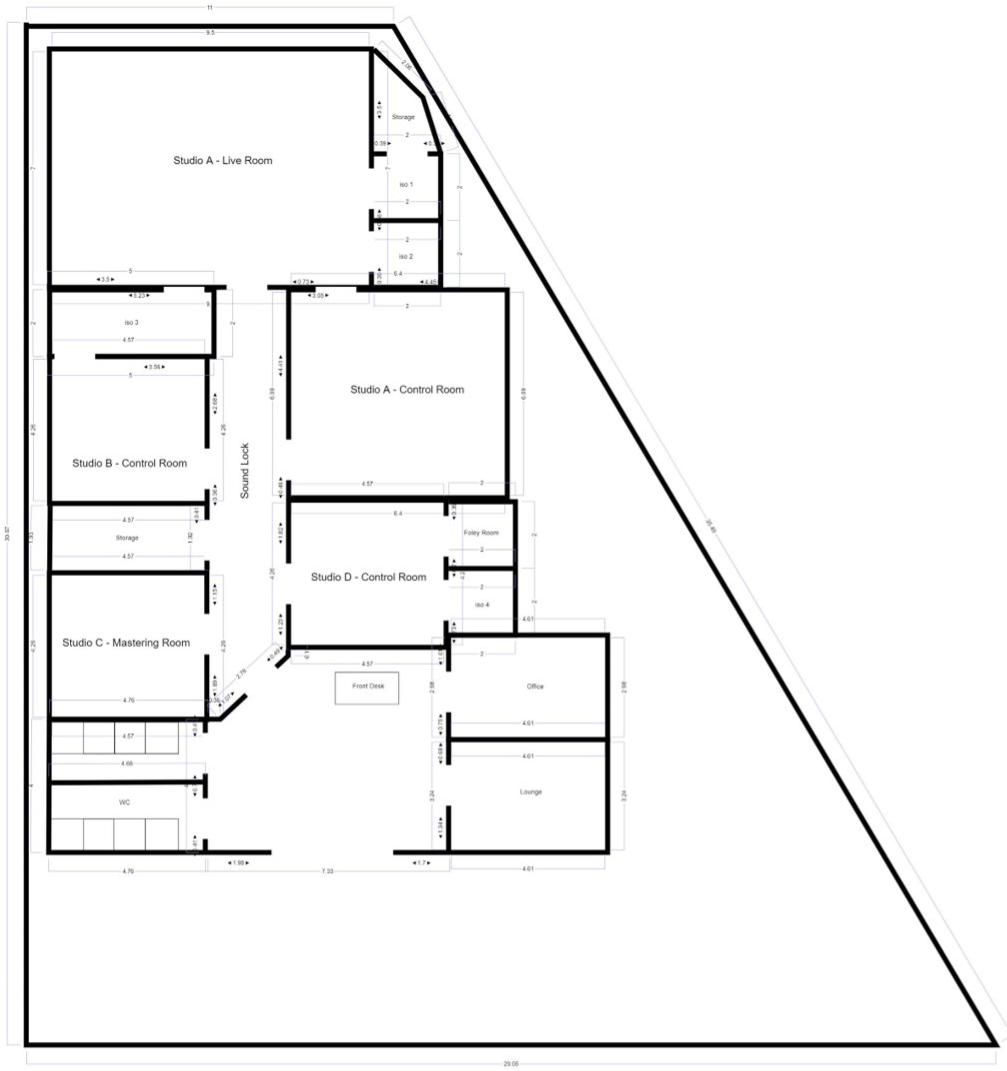
\includegraphics[scale = 0.8]{resources/floorplan.png}}
            \caption{The floor plan of the music educational facility}
            \label{floorplan}
        \end{figure*}
        With only one regular point of entry and exit, any entrances or exits made by students or staff can be monitored, such that issues with missing equipment or safeguarding concerns can be easily managed.
        Studio A has a transparent viewport into the live room.
        Thus, it can be used as a control room for any large ensemble recording, such as an orchestra.
        The same applies for the viewport between iso room 3 and the live room.
        It is important to consider the AV-over-IP networking technology used by the studio; it allows for fluid redirecting of the signal chain in a recording environment.
        For example, the live room can be also be used as a control room for a recording in iso room 3, with minimal adjustment to the hardware present in either room.
        All that may need to be changed is the software patching of the AV-over-IP.
        This further allows any student to become proficient in using AV-over-IP technology, a fast advancing technology in the modern studio.
    \section{Interior Acoustic Design}
        \subsection{Introduction}
            When designing rooms for optimal interior acoustic performance, we must take into account the frequency-based and reverberant performance of the room.
        \subsection{Reverberance}
            The reverberance of a room is quantified in the form of an $RT_{60}$.
            The value of a room's $RT_{60}$ defines the time taken for an acoustic impulse's (a short, fast transient, loud sound) SPL to decay by 60dB.
            To calculate the RT60 of a cuboid room, Sabine's equation is most often used:
            \begin{equation}\label{sabines}
                RT_{60} = \frac{0.161 V}{A}
            \end{equation}
            Where $V$ is the volume of the room, and $A$ is the total absorption of the walls, ceiling and floor.
            As different rooms within the complex have intended use cases, they will require a variety of $RT_{60}$ values, depending on said use case.
            For example, as the live room needs to have a natural, projecting and reverberant sound such that large ensembles blend together and a teacher can speak to the entire room with ease, it needs to have a larger $RT_{60}$ than other rooms.
            Comparatively, the control rooms and isolation rooms will have a much lower $RT_{60}$.
            The values of $RT_{60}$ for each room are tabulated in Fig.\ref{RT60}
            Rearranging Eq.\ref{sabines}, we can solve for each room's $A$:
            \begin{equation}
                A = \frac{0.161V}{RT60} 
            \end{equation}
            \begin{figure}[H]
                \centering
                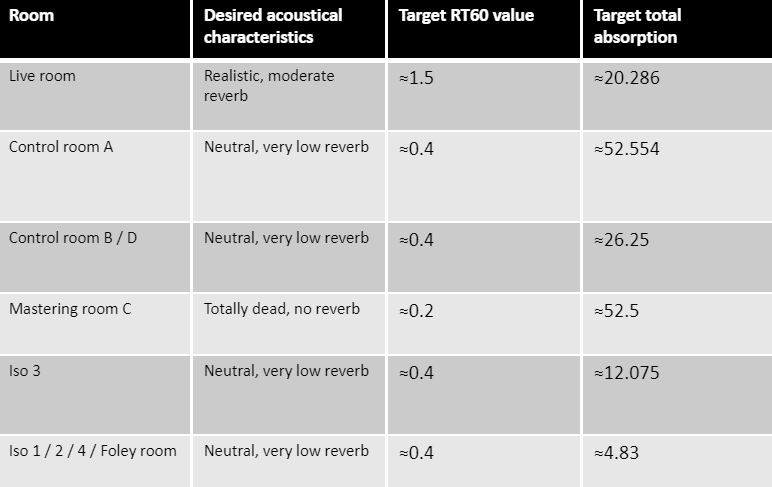
\includegraphics[scale=0.48]{resources/RT60.png}
                \caption{Table of target RT60s and total absorption for each room}
                \label{RT60}
            \end{figure}
            Taking these target total absorptions, we then calculated the required contribution from each surface to the total absorption of each room using an Excel spreadsheet.
            To find the contribution of a surface, the absorption coefficient of it's material must be multiplied with it's surface area.
            Different construction materials have different absorption coefficients, and as such the material of each surface must be chosen in order to dial in the correct contribution to total absorption from the surface.
            The materials chosen, absorption contributions and total absorption of each room are tabulated in Fig.\ref{reverb}.
            \begin{figure*}
                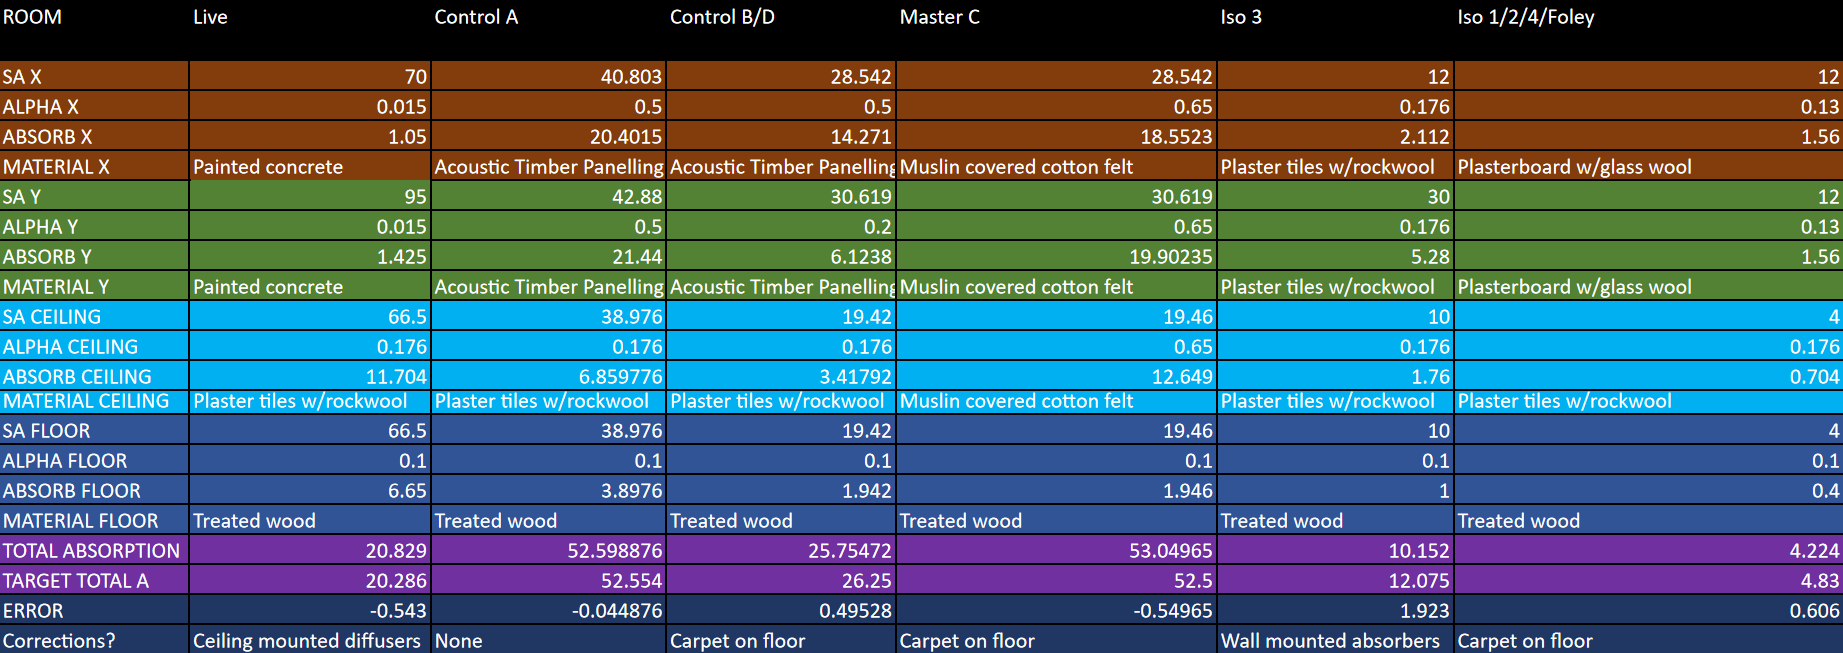
\includegraphics[scale=0.4]{resources/reverb.png}
                \caption{Table detailing room construction to achieve room's target $RT_{60}$}
                \label{reverb}
                \centering
            \end{figure*}
        \subsection{Room modes}
        Room modes are a common problem in sensitive acoustic environments, and thus there is a great deal of research and literature regarding their suppression.
        Specifically designing the dimensions of rooms, and the proportions between them, to certain values helps target and suppress common room modes.
        The optimal methodology of determining room proportions is described in \cite{Cox}. With the help of an computer algorithm, the proportions that produce the flattest modal frequency response can be found using this method.
        For this project, the room proportions were determined according to the ratios obtained by Eq.\ref{ratios}
        \begin{equation}\label{ratios}
            f = \frac{c}{2}\sqrt{(\frac{n_x}{L_x})^2+(\frac{n_y}{L_y})^2+(\frac{n_z}{L_z})^2}
        \end{equation}
        and then the room modes were calculated in order to take acoustic treatment measures.
        There are several previous methods developed by different acousticians such as Bolt\cite{Bolt} and Gilford\cite{Gilford}.
        The ratios in Fig.\ref{bolty}, which use Bolt's method, was used for the small rooms in the design.
        \begin{figure}[H]
            \centering
            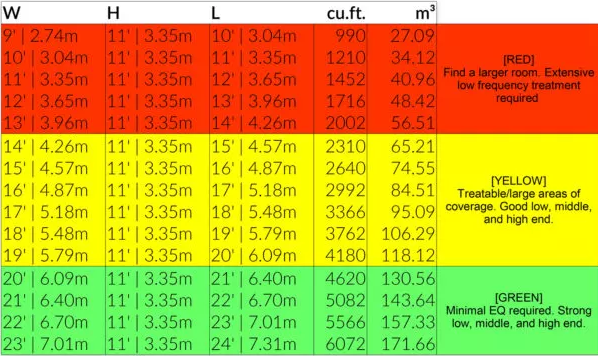
\includegraphics[scale=0.5]{resources/modey.png}
            \caption{Our chart of acceptable proportions}
            \label{bolty}
        \end{figure}
        Cuboid rooms can facilitate standing waves, which can lead to problems with uneven frequency response throughout the room, and thus an uneven listening experience.
        This uneven characteristic is caused by the nodes and anti-nodes of the standing waves not moving in space; the locations of the nodes are known as 'room modes'.
        A standing wave is a wave travelling through a medium, in this case the air, oscillating in time.
        However, due to the distance between the boundary conditions being an integer multiple of the incident wavelength, after reflecting when reaching the boundary conditions of the medium, it appears to not oscillate in time, due to the constructive or destructive interference of the incident and reflected wave \cite{PHYS15}.
        In order to predict the frequencies at which standing waves will appear, the X-Y-Z dimensions of the room are taken as integer multiples / factors of the standing wave frequencies.
        Thus Eq.\ref{standing} can be solved for $f_n$, where $n$ is the harmonic number of the standing wave, $c=343\si{\meter\per\second}$ is the speed of sound in air, and $L$ is the length of the dimension in question.
        \begin{equation}\label{standing}
            f_n = \frac{c}{2L}n
        \end{equation}
        This equation will only solve for axial room modes; an acoustic wave in three-dimensional dimensional space does not only reflect back unto it's self, but also at various angles of reflection.
        These angular second and third reflections of an axial room mode are known as tangential and oblique room modes, as shown in Fig.\ref{oblique}.
        \begin{figure}[H]
            \centering
            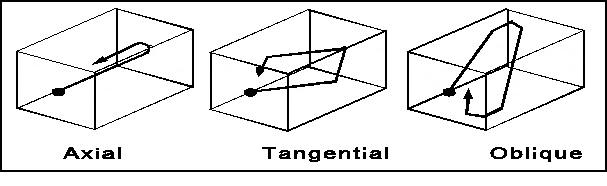
\includegraphics[scale=0.375]{resources/oblique.jpg}
            \caption{An illustration of three types of room mode \cite{MODES}}
            \label{oblique}
        \end{figure}
        Using Excel and Eq.\ref{standing} frequency values for axial room modes on the X-Y-Z axis up to the 9\textsuperscript{th} harmonic were calculated; the full tabulated results can be found in Fig.\ref{modes}
        \begin{figure*}[ht]
            \centering
            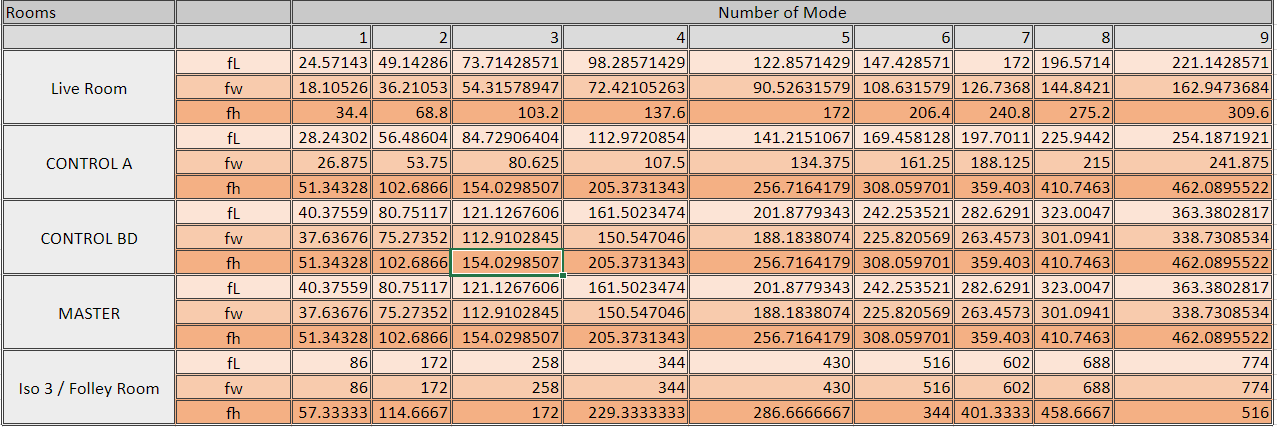
\includegraphics[scale=0.6]{resources/modes.png}
            \caption{Table detailing axial room modes for each room}
            \label{modes}
        \end{figure*}
        We then moved on to the issue of dealing with the found room modes.
        The room modes with the greatest impact on the even listening field are towards the lower end of the frequency spectrum; the number of nodes in a standing wave of 5cm wavelength in a room 9m wide makes it's effect inconsequential, whereas a wave with a 4.5m wavelength will only two locations in the room where it reaches it's true peak amplitude.
        In order to prevent these frequencies becoming standing waves, we must target them for absorption.
        Resonant membrane absorbers are very useful in this context - they provide relatively precise targeting and attenuation of problematic frequencies.
        Eq.\ref{membrane} formulates how to solve for the depth and mass of a membrane absorber to target a certain frequency, where $d$ is depth, $m$ is mass per meter square, and $f$ is frequency:
        \begin{equation}\label{membrane}
            f = \frac{60}{\sqrt{md}}
        \end{equation}
        Setting $m=1\si{\kilogram\per\meter\squared}$ for ease of production allowed us to simply solve for a $d$ that would cause the membrane absorber to target the first room modes of each room
        \begin{figure}[H]
            \centering
            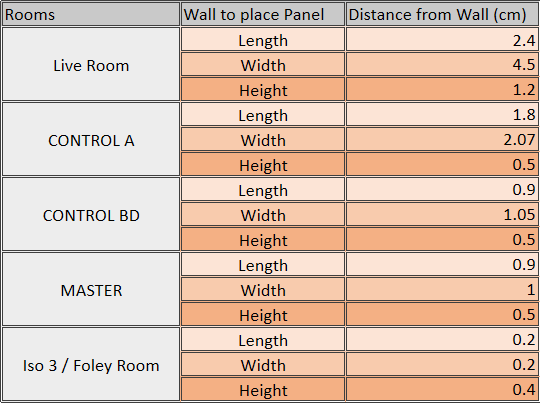
\includegraphics[scale=0.7]{resources/membrane.png}
            \caption{Table detailing the depths of membrane absorbers used to target first harmonic room modes}
            \label{membranetable}
        \end{figure}

    \section{Noise Insulation}
        \subsection{Introduction}
            'Noise' can be characterized as any unpleasant or unwanted sound.
            Typical sources of noise in the general built environment can include road traffic noise, ground vibrations from passing trains, electrical plant noise, and airplanes passing overhead.
            It is possible, and highly likely in a recording studio environment, that the sound that one person thinks as desirable or pleasant, to be considered an extreme nuisance by another in the building.
            Unwanted noise both from within the studio and from without is an issue of great consideration for recording studios.
            A potentially perfect take can be ruined by microphone bleed of a truck passing by or an underground train shaking the floor.
            Noise reduction (NR) curves dictate the maximum acceptable noise level in a room over the audible frequency spectrum.
            Different NR number indicate different acceptable levels of noise.
            As the studio is a particularly sensitive acoustic environment, a strict NR number of NR10 was chosen.
            
        \subsection{Sound Reduction Index}
            Sound reduction index (SRI) measures the ratio at which sound waves are attenuated upon transmission through a solid body \cite{REDBOOK}.
            This reduction ratio is expressed in decibels, shown in Eq.\ref{SRI} where $W_r$ is sound energy on the receiving side of a body, and $W_s$ is the energy on the source side:
            \begin{equation}\label{SRI}
                SRI = 10\log{\frac{W_s}{W_r}}
            \end{equation}
            Sound reduction through a solid body is not constant across all frequencies.
            Taking into account the chosen NR10, and solving for SRI, we could calculate SRIs for each octave band.
            Using MATLAB, SRI values across the frequency spectrum were calculated and plotted for an outside-to-inside and inside-to-inside sound transmission, as shown in Figs.\ref{MATLAB1}\&\ref{MATLAB2}:
            \begin{figure}[H]
                \centering
                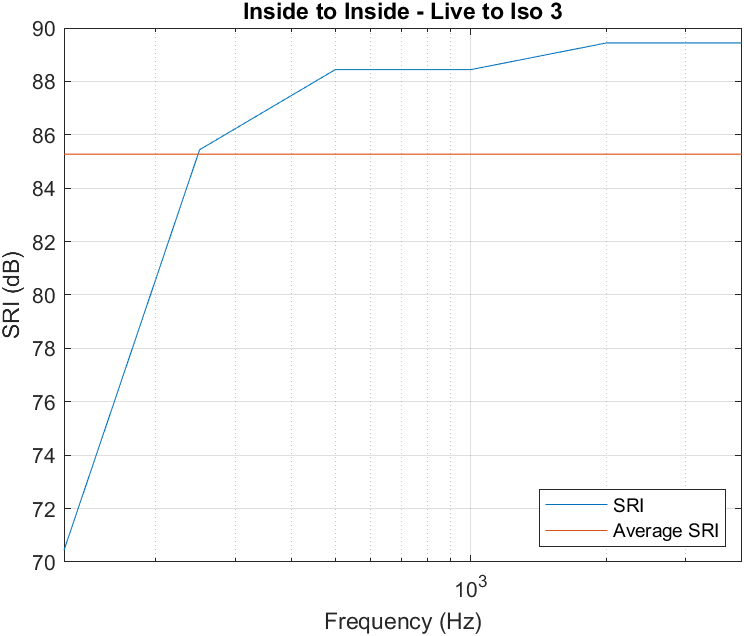
\includegraphics[scale = 0.6]{resources/I2ILive2Iso3.png}
                \caption{Inside-to-inside SRI over frequency}
                \label{MATLAB1}
            \end{figure}
            \begin{figure}[H]
                \centering
                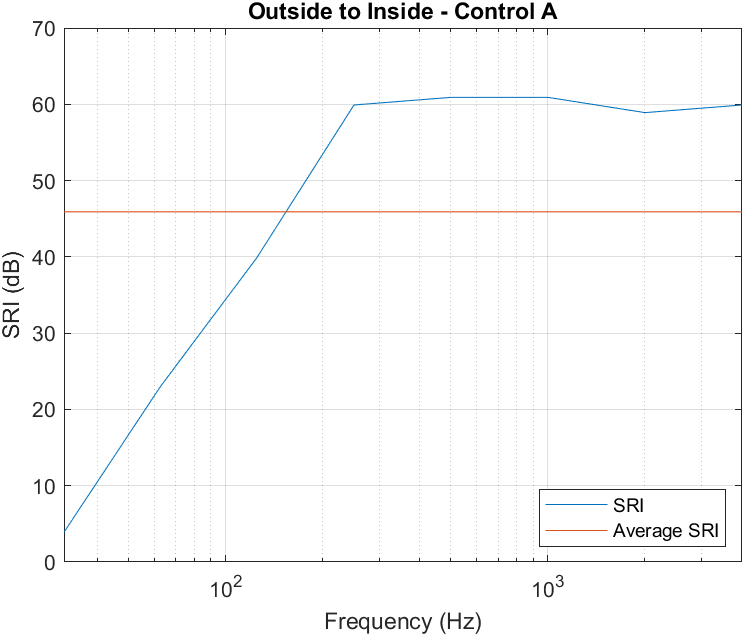
\includegraphics[scale = 0.6]{resources/O2IControlA.png}
                \caption{Outside-to-inside SRI over frequency}
                \label{MATLAB2}
            \end{figure}

        \subsection{Methods of Insulation}
            The most effective method for preventing noise from entering a room is designing the structure of the room such that the vibrations travelling through solids and sound waves causing said unwanted noise are prevented from entering the structure.
            This can prove challenging, as acoustic waves can travel through almost any solid of a reasonable structural thickness, and a solid structure is by far the easiest and most common way to design the built environment.
            In anechoic chambers found in acoustic research institutes, rooms are suspended from large mass dampers within rooms, with the chamber having a completely separate set of foundations from the rest of the building. REF.
            This construction and design, whilst incredibly effective at reducing outside noise from coming into a room, is very costly and restrictive.
            Instead, our studio was acoustically designed with the aim of reducing outside noise, whilst still providing a familiar built environment.
            Elements we considered included: Absorption, damping, decoupling and distance.
            Absorption of unwanted noise can be achieved by placing acoustic insulation between each wall section, as illustrated in Fig.\ref{wallFiller}.
            \begin{figure}[H]
                \centering
                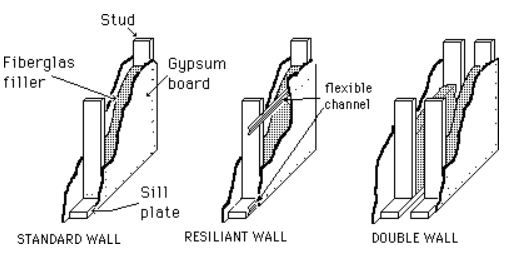
\includegraphics[scale = 0.6]{resources/wallFiller.png}
                \caption{Filling wall partitions with acoustic insulation \cite{UCSC}}
                \label{wallFiller}
            \end{figure}
            Decoupling the superstructure of the building from the outside world was achieved by planning large mass dampers ('springs') into the support structure, as seen in Fig.\ref{springs}:
            \begin{figure}[H]
                \centering
                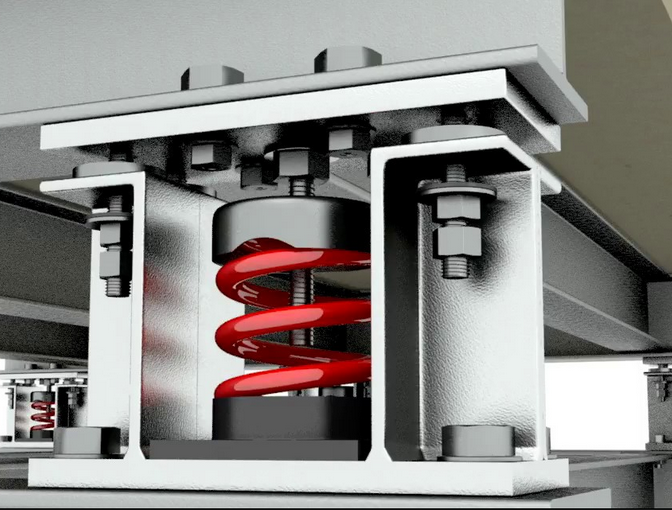
\includegraphics[scale = 0.5]{resources/springs.png}
                \caption{Large structural springs used to decouple rooms from the superstructure}
                \label{springs}
            \end{figure}

    \section{Studio Layout}
            Each studio is equipped with modern, state-of-the-art equipment, in a modular fashion such that they can be easily tweaked and adjusted.
            As previously mentioned, AV-over-IP is used to interconnect equipment between every room.
            To elaborate: Audinate's Dante system is used, along with Focusrite RedNet Dante networking switches.
            Each RedNet acts as a terminal to connect a piece of digital equipment to the Dante network.
            Interconnections between devices are made using Cat5 cables, of various custom lengths to provide clean cable runs.
            Room for extra connections are to be kept free on every RedNet, such that a student or member of staff may make extra interconnections as they wish.
            A comprehensive network diagram was made, shown in Fig.\ref{network}
            \begin{figure}[H]
                \centering
                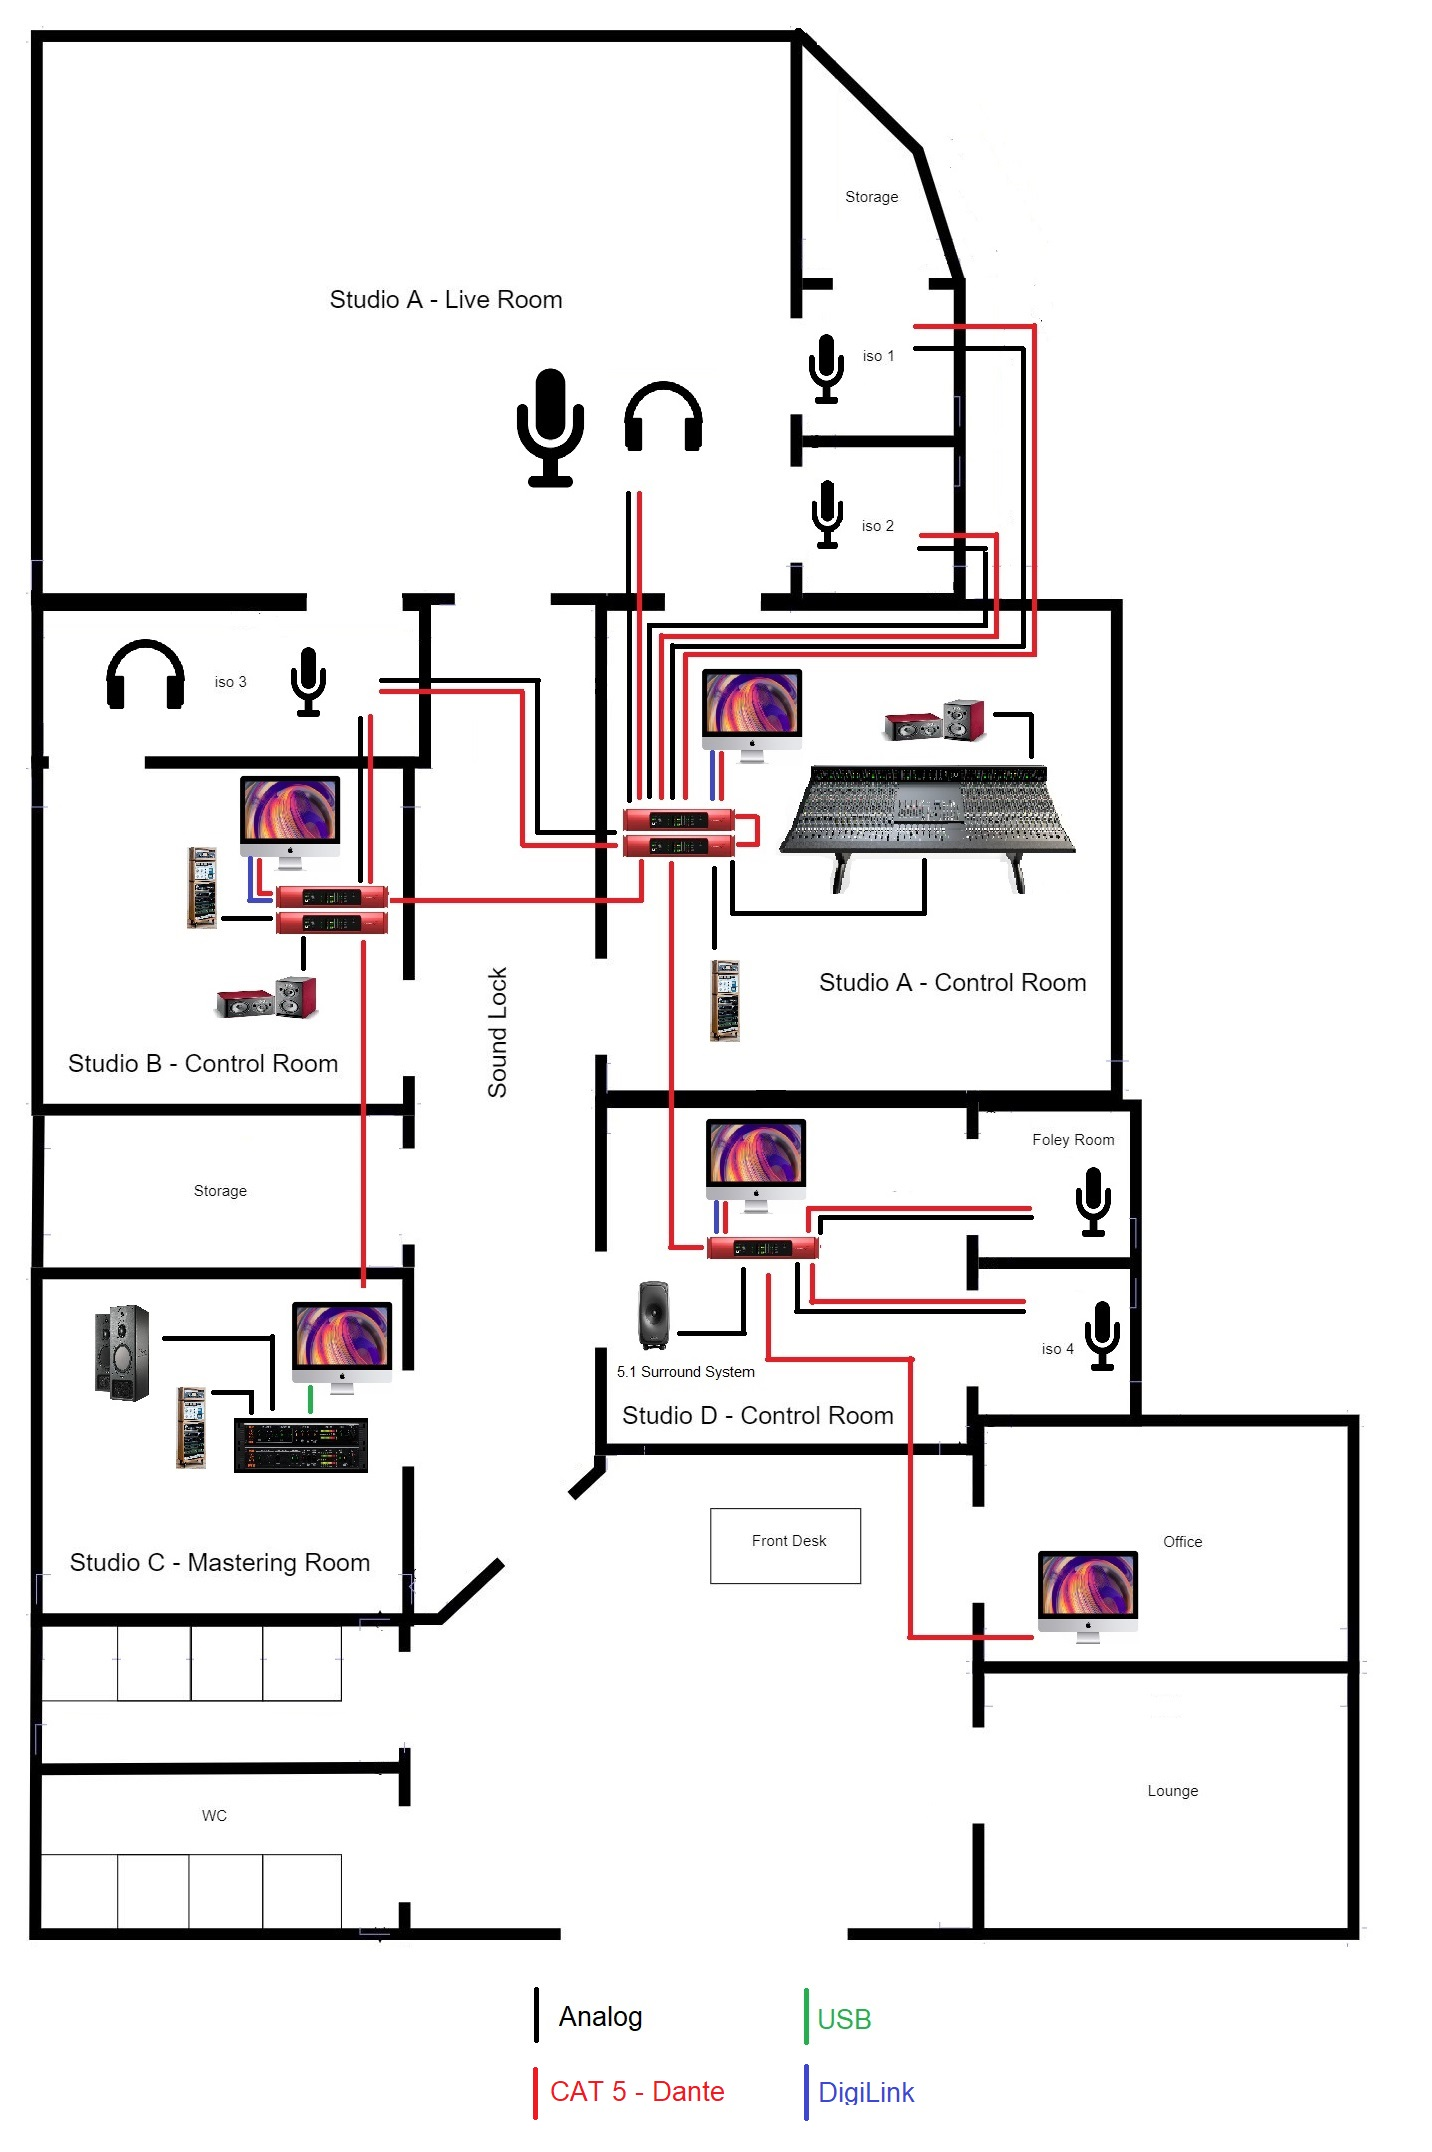
\includegraphics[scale=0.2]{resources/network.png}
                \caption{Network diagram for the studios}
                \label{network}
            \end{figure}
            A seen in Fig.\ref{network} there are also DigiLink and USB connectivity available.


    \section{Conclusions}
        In conclusion, the acoustic considerations for each room have been thoroughly considered.
        However, the impact of suggested noise insulation measures, for example the spring-based supports, were not explored or investigated.
        Furthermore, SRIs were only found for two solid barriers, and whilst they may have given a good indication of the performance of all the solid barriers and walls, they do not illustrate their performance for certain.
        As such further investigation in to the SRI performance between every separate would have served to guarantee the prevention of any noise problems.
        Also, whilst porous absorbers are suggested to correct total absorption errors illustrated in Fig.\ref{reverb}, no explanation was given as to the type of porous absorber suggested nor the frequency performance of said absorbers.
        Research in to local council requirements and utility costs would have served to improve the detail of the case study.

    \bibliographystyle{plain}
    \bibliography{theBib}
\end{document}